\chapter{Applications of QOCT to Many-Body Quantum Systems}

A wide variety of experiments utilizes the properties of the Mott Insulator, which is produced by initially loading a Bose-Einstein condensate into a single trap followed by slowly ramping up a periodic lattice potential. As the lattice depth increases, a quantum phase transition between the Superfluid and the Mott Insulator takes place. This sequence is a necessary first step for many experiments \cite{manybodyBloch}. In order to perform such experiments a very low number of defects in the final state is required, thus people have resorted to adiabatic transitions, where one varies the lattice depth slowly across the critical point, such that the system remains in the ground state with sufficiently high probability. Naturally this comes at the cost of the sequence being quite slow - typically performed in about a hundred milliseconds \cite{JakschZoller}.\\
Preparing the Mott Insulator state at a faster rate is very desirable, as it allows faster data acquisition as well as lowers the timespan in which de-coherences and defects can be introduced through interactions with the environment. However, faster transitions can only be achieved non-adiabatically, hence numerical simulations are critical in the investigation due to the exponential growth of the Hilbert space near the critical point \cite{Vidal2003}.

\section{Methods of Optimization}

Calculating a non-adiabatical ramp of the lattice potential, which reaches a final state with sufficiently low defect, was made possible with the unification of the quantum optimal control theory and the tDMRG algorithm \cite{Doria2011,FrankBloch}. In both cases the optimization method used is the Chopped RAndom Basis (CRAB), where one is looking for a control field of the form
\begin{equation}
	V(t) = V_0 (t) f(t),
\end{equation} 
where $V_0 (t)$ is an initial guess (often based on either physical intuition of the problem or preexisting solutions), and $f(t)$ is a correction expressed in a truncated and randomized basis. A popular choice is a truncated Fourier series of the form
\begin{equation}
	f(t) = \frac{1}{N} \left[ 1 + \sum_{k = 1}^{M} A_k \sin(\nu_k t) + B_k \cos(\nu_k t) \right] \; ,
\end{equation}
where $M$ is the basis size, $\nu_k = 2 \pi k (1 + r_k )/T$ are the Fourier harmonics with $r_k \in [-1/2 , 1/2]$ being random uniformly distributed, and $N$ is a normalization constant for keeping the initial and final control pulse values fixed \cite{Doria2011}. Thus, one can reformulate the optimization problem as the extremization of the multivariable function $\mathcal{F}(\{ A_k \}, \{ B_k \}, \{ \nu_k \})$. Solving this new problem can be done using either direct search methods like Nelder-Mead \cite{NumericalRecipes} or gradient based methods \cite{Winckel2008}.

\section{Numerical Results and Experimental Realization}
Numerical optimization of the lattice potential ramp was performed and experimentally tested in \cite{FrankBloch}. The system considered in the article is the standard Bose-Hubbard model with the addition of an underlying harmonic confinement potential. Thus, the Bose-Hubbard Hamiltonian in question reads
\begin{equation}
\hat{H} = - J \sum_{\langle i,j \rangle} \hat{a}_{i}^{\dag} \hat{a}_{j} + \frac{U}{2} \sum_{i} \hat{n}_i \left( \hat{n}_i -1 \right) + \frac{1}{2} m \omega^2 a_{\mathrm{lat}}^2 \sum_{i} \left( i - i_0 \right) ^2 \hat{n}_i \; ,  \label{eq:BHtrap}
\end{equation}
where $i_0 = (L -1)/2$ is the center of the trap. $\omega = 2 \pi \times 63.5 \mathrm{Hz}$ was chosen to match that of the experiment. The lattice used for both the calculations and the experiment was 32 sites long and contained 16 particles. Thus, as the phase transition occurs, one would expect the Mott Insulator to form in the central 16 cites due to the underlying harmonic potential. Although not stated explicitly, the choice of using a half filling fraction was presumably to avoid boundary effects, as these can have an influence on the location of the critical point of the phase transition \cite{Kuhner2000}. Furthermore, the figure of merit was defined as
\begin{equation}
	F(t) = \frac{1}{8} \sum_{i = L/2 -3}^{L/2 +4} \frac{\Delta n_{i}^2 (t)}{\Delta n_{i}^2 (0)} \; , \label{eq:FMerit}
\end{equation}
where $\Delta n_{i}^2 (t) = \braket{\hat{n}_{i}^2 (t)} - \braket{\hat{n}_{i} (t)}^2$ was the rescaled variance of the population of site \textit{i}. This figure of merit measures this rescaled variance of the 8 most central sites, where the effect of the underlying harmonic potential is minimal. Although the motivation for choosing this figure of merit as opposed to the infidelity, which is the standard choice, is not stated in the article, one may assume it being related to experiments, as the variance in the site occupancy of a Mott Insulator is relatively easy to measure. The initial state of the system yields $F(t=0) = 1$, while a pure Mott-Insulator yields $F = 0$, where any fluctuations or residual excitations will result in an increase of $F$.\\
The Bose-Hubbard model is only truly valid within the tight binding limit ($V \approx 5-8 E_r$), where the Wannier functions are sufficiently localized, such that only nearest-neighbor interactions are allowed. However, as backed up by the experimental results of \cite{FrankBloch}, applying the Bose-Hubbard model to lattice depth as low as $V = 3 E_r$ can produce accurate results. Hence, in this instance an initial, non-optimized ramp to $V = 3 E_r$ was performed followed by a ramp to $V = 14 E_r$. This final lattice which is deep into the Mott regime, as the critical point for the phase transition without a harmonic confinement is around $V_c = 4.5 E_r$ \cite{Kuhner2000}.
\begin{figure}[h!]
	\centering
	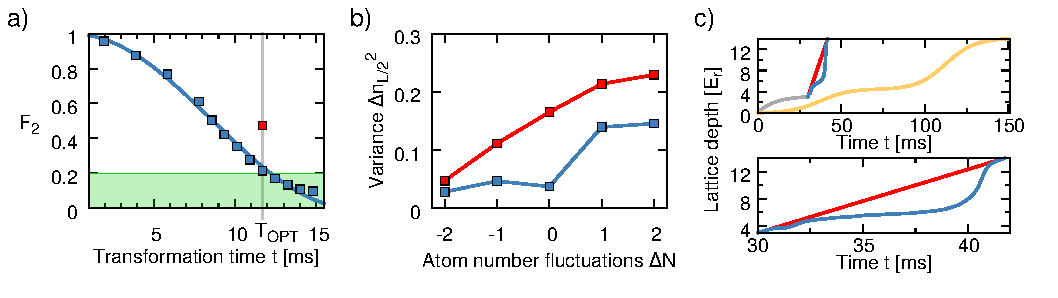
\includegraphics[width=0.9\textwidth]{Figures/FrankRamp.pdf}
	\caption{\textit{Numerical results from \cite{FrankBloch}. (\textbf{a}) Figure of merit for optimized pulse. The green region marks the experimental infeasible region. (\textbf{b}) Theoretical prediction for atom number fluctuations in the center of the trap for various deviations from 16 particles. (\textbf{c}) Comparison between a fast linear ramp (red), the optimized ramp (blue), and a typical adiabatic ramp (yellow). The initial slow ramp to $V = 3 E_r$ is shown in grey.}}
	\label{fig:FrankRamp}
\end{figure}\\

The results of the numerical optimization of \cite{FrankBloch} are displayed in figure \ref{fig:FrankRamp}. The figure of merit (equation \ref{eq:FMerit}) for the optimized pulse is displayed in figure \ref{fig:FrankRamp}.a along with the corresponding value for a fast linear ramp at the time $t = T_{\mathrm{OPT}}$ (marked with a red square). Clearly the optimized ramp produces a much better figure of merit compared to the linear ramp. As stated in \cite{FrankBloch} the curve shows the expected shape $F(t)= \cos^2\left(t/T_{\mathrm{QSL}}\right)$ for an optimal crossing of a quantum phase transition \cite{Caneva2011}, however, this universality has only been shown in scenarios of the figure of merit being the infidelity. Whether the cosine expression also universally applies to other figures of merit remains to be shown. The cosine fit yields a quantum speed limit of $T_{\mathrm{QSL}} = 17.3(2) \mathrm{ms}$. In figure \ref{fig:FrankRamp}.b the atom number fluctuation at the center of the trap is displayed for the two fast ramps for various number of particles. At 16 particles the optimized ramp clearly outperforms the reference linear ramp. Finally, figure \ref{fig:FrankRamp}.c displays the actual shape of the ramps.\\

Experimentally applying the ramp acquired through numerical optimization lead to an average site occupancy of 0.80 in the central sites of the trap. These defects were mainly attributed to a finite temperature of the initial state. This experimental limitation is illustrated in figure \ref{fig:FrankRamp}.a by the green shaded region and was reached after a ramp time of $T_{\mathrm{OPT}} = 11.75 \mathrm{ms}$.\\
Thus, as \cite{FrankBloch} demonstrated, it is indeed possible to achieve the SF-MI transition through a non-adiabatic ramp, while simultaneously ending up in the ground state of the system.